\section{Builder}
\label{sec:builder}
As mentioned in previous sections, miq has a 2-stage package
evaluator that produces a dependency graph of Units in
memory. This dependency graph is consumed during the build
process, executing the script of each Package Unit or
fetching the necessary files of Fetch Units.

\subsection{Sandbox}

Fetch Units are trivially built, as it is only needed to do
an HTTP request to the selected |url|, and store the
resulting file into the store path. Optionally, the user
might select to change the permissions of the file to be executable.

Package Units use a more involved process. To begin with,
they are built in a build sandbox. The purpose of the
sandbox is to isolate the execution of the script from the
outside world. This means that the process only sees a
limited view of the file system and network connection is
limited. The sandbox isolates the file system by only giving
the process views on essential paths, like |/dev|, |/proc|
or |/tmp|. A view on |/miq/store| is also allowed, and the
build scripts contain absolute paths into it. For this
reason, it does not matter what the existing content of the
store is from one machine to another, as only the
``hardcoded'' paths into the dependencies are used. The
development model of miq by hashing every package to provide
a unique path completely bypasses the need to selectively
mount specific packages into the build sandbox. To create
this sandbox, miq relies on Linux namespaces
\cite{NamespacesLinuxManualb} . Linux namespaces are an
interface provided by the kernel itself, to change
resources of a process. The resources that can be changed
include: mount points, user IDs, network, etc. While
initially miq leveraged directly the namespaces interface
via the |libc| crate, it was later changed to run the
program bubblewrap as a subprocess . Bubblewrap \cite{Bubblewrap2023} is a C
application that wraps the namespaces interface with a
\ac{CLI}, such that the user can easily run processes in a
sandboxed environment. Therefore, miq calls bubblewrap with
the appropriate flags to provide a build sandbox for the
build script.

The usage of a sandbox is crucial for the reproducibility of
the package builds. The development model of miq assumes
that a package is uniquely identified by its hash, which in
turn is derived from its inputs (build script and
dependencies). If the package produces a result that is not
reproducible, this means that a same hash potentially points
to different results -- from one computer to another or
rebuilds in the same computer. Some sources of
``impurity'' are:

\begin{enumerate}
    \item Environment variables
    \item User ID, name and groups
    \item Files that are not part of the miq store, like
    |/etc|, |/home|, |/var|, etc.
    \item Network connection (e.g. fetching from the
    internet might fail or give different results)
\end{enumerate}

Environment variables are trivially cleaned by any
subprocess invocation. Miq additionally inserts some extra
environment variables, like |\$miq_out|, which points into
the output directory or |\$HOME| pointing to the build
directory.

To isolate the user ID, user namespaces are used. User
namespaces allow to create a mapping of user IDs outside the
sandbox into user IDs in the sandbox. In practice, the user
running miq is mapped into the root user. The child process
``sees'' that it is running as root, while it is being
executed on behalf of the user (with all the limitations and
permissions of the user, not of root).

The file system can be isolated by using a mount namespace.
It allows to mount a new root |/|,
and then selectively mount the necessary paths into this
blank slate. Some core paths are required, such as |/dev| or
|/proc| to even be able to run any application. A mapping of
a build directory into the sandbox at |/build| is created.
It is also possible to mount |/miq/store| as read-only, such
that the build script is not able to modify any existing
package by accident.

Finally, the network connection can be trivially
disconnected by using network namespaces and the appropriate
flags to bubblewrap. As mentioned before, Fetch Units are
not built in a sandbox and rely on fetching files from the
internet, which can potentially produce impure,
non-deterministic results. This can be avoided by using a
resource-integrity mechanism
\cite{chapuisEmpiricalStudyUse2020} . What this would
involve is checking that the received content matches
against an already-known hash, that is derived from the file
contents. The hash can be manually calculated by \acl{TOFU}
and written in the package definition. This is currently not
implemented into miq, but it is a planned feature.

\FloatBarrier
\subsection{Concurrency}
\label{sec:concurrency}

As the source-based package managers NixOS' nix and
Gentoo's emerge, miq is able to build package in parallel. A
parallel build process implies that there the build is not
sequential. In a sequential (or 1-job build), every package
is built one after the other, waiting for the previous in
the line to build the next one. Considering that the
structure used to represent the dependency graph is a
\acl{DAG}, on first iteration one solution is to compute the
topological sort of the graph
 . This sort
involves converting the graph into a sequence of nodes, such
that the ordering between the nodes is preserved
\cite{erParallelComputationApproach1983} . Finally, a
builder can travel the sequence to build each dependency in
order on after the another.
This process is not efficient, as a package only requires
that its dependencies are built, but not every node in the
topological sort. Figure \ref{fig:toposort} shows an example
of a topological sort of a simple package that depends on 2
Fetch Units. In this situation, only when one of the Fetch
Unit finalizes the transaction, which involves downloading
the file from the internet and saving it to the disk, can
the next Fetch Unit start its process.

\begin{figure}[hbtp]
    \centerfloat
    \includesvg[width=280pt]{assets/toposort.svg}
    \caption{Topological sort of a \ac{DAG} with 2 Fetch Units.}
    \label{fig:toposort}
\end{figure}

A more complex example of how a topological sort is not
desired is shown in figure \ref{fig:toposort2} . As can be
seen, Package B must wait until Fetch B has finished, while
all its dependencies (just Fetch A) has already been built.
Similarly, Package C must wait until Package B has been
built. As a result of the definition of a topological sort
being a sequence of nodes where ordering is respected, all
the edges in the topological sort point ``upwards'' into the
root unit. Cyclic graphs cannot be topologically sorted, as
the ordering cannot be preserved, and we would need to build
a package as a dependency of itself, as displayed on figure
\ref{fig:toposort3} .

\begin{figure}[hbtp]
    \centerfloat
    \includesvg[width=300pt]{assets/toposort2.svg}
    \caption{Topological sort of a \ac{DAG} with 2 Fetch and
    2 Package Units.}
    \label{fig:toposort2}
\end{figure}

\begin{figure}[hbtp]
    \centerfloat
    \includesvg[width=300pt]{assets/toposort3.svg}
    \caption{Impossible topological sort of a directed cyclic graph.}
    \label{fig:toposort3}
\end{figure}

\FloatBarrier

A builder that uses topological sort can be easily
implemented, as the library that provides the \ac{DAG}
structures also provides the method in
|daggy::petgraph::algo::toposort|. While miq used this
sequential approach initially, it was developed a new
algorithm to perform the builds concurrently. To properly
track the Units that have been built or not, the following
|enum| is used:

\begin{minted}{rust}
enum BuildTask {
    Waiting,
    Building,
    Finished,
}
\end{minted}

To begin with, every Unit gets attached a new |BuildTask| by
creating a simple map of the list of Units to their state.
Every Unit starts in the |Waiting| state.

\begin{minted}{rust}
let mut build_tasks: HashMap<&Unit, BuildTask> = HashMap::new();
\end{minted}

Then, an iterative process is started, following the steps:

\begin{enumerate}
    \item Scan all the Units in the \ac{DAG}. For every Unit U do:
    \begin{enumerate}
        \item Scan all of U's dependencies. If all of them
        are |BuildTask::Finished|, or if there are no dependencies,
        then U can be built.
        \item Spawn a new thread to build U, and mark it as
        |BuildTask::Building| in the map.
    \end{enumerate}
    \item Wait for any thread to finish. If the tasks is OK,
    mark it as a |BuildTask::Finished|. If any errors occur,
    return them and stop any other tasks.
    \item If all tasks are |BuildTask::Finished|, return.
    Otherwise, loop back to the first step.
\end{enumerate}

Overall, the algorithm scans the \ac{DAG} in an infinite
loop, spawning threads to build the Units, as soon as
they can be built. This happens when all of a Unit's
dependencies have finished.

Rust's asynchronous ecosystem is leveraged to be able to
spawn threads that don't block. The asynchronous runtime
used for this task is Tokio \cite{TokioRust}, as the Rust
language only provides the primitives to declare
asynchronous functions on the type level, but doesn't
provide any runtime to execute them. Tokio and the async
Rust ecosystem is based on the concept of green thread. A
green thread is a thread that is not executed by the
operating system, but rather by a runtime (in this case,
Tokio). A green thread runtime uses its available CPU time
to context-switch between a list of tasks that are waiting.
Whenever a task is being executed, it is the only task that
the runtime executes -- without any parallelism -- until the
task hits an |await| point. Then, the runtime switches the
context to another tasks that is waiting, until that one
also hits an await point. The process is repeated until all
tasks have finished. Thus, the runtime is only executing a
single task at any instant of time, but the context
switching between tasks provides the illusion of the tasks
being executed in parallel, as shown in figure \ref{fig:timeshare} .

\begin{figure}[hbt]
    \centerfloat
    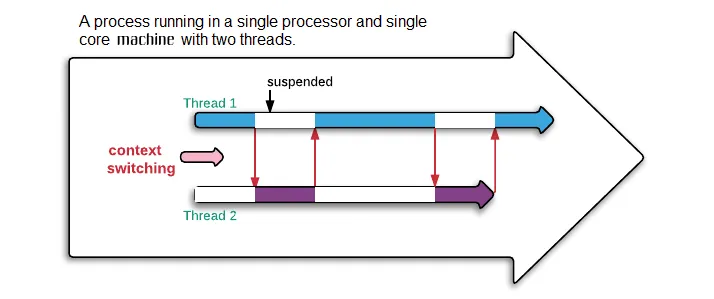
\includegraphics[width=350pt]{assets/timeshare.png}
    \caption{Context switching between tasks in a green thread runtime.}
    \label{fig:timeshare}
\end{figure}

Tokio also provides a hybrid approach to threads, as it uses
a thread pool to execute the tasks. The thread pool is
mapped into operating system threads, so the tasks can be
run in parallel if the runtime decides to put them into a
different backing \ac{OS} thread.

However, a parallel runtime is not needed for miq, as the
build tasks are spawned as a subprocess for bubblewrap, the
build sandbox discussed in the previous subsection. Every
task executes bubblewrap, which gets a new \acl{PID} and is
executed by the OS apart from the thread runtime. Thus, the
tasks executed by miq only collect the logs generated by the
bubblewrap subprocesses, which happens concurrently.

\begin{figure}[hbt]
    \centerfloat
    \includesvg[width=350pt]{assets/parallel.svg}
    \caption{Concurrent process to build 5 Units.}
    \label{fig:parallel}
\end{figure}

Figure \ref{fig:parallel} shows an example of how this
algorithm schedules the builds such that every Unit is built
as soon as every dependency has been built. The colors for
the figures indicate:
\begin{itemize}
    \item White: |BuildTask::Waiting|
    \item Yellow: |BuildTask::Building|
    \item Green: |BuildTask::Finished|
\end{itemize}

The process is as follows:

\begin{enumerate}
    \item Units E and D have no dependencies, so they are built first.
    \item D finishes, so C can be built now. A build task is
    spawned for C.
    \item E finishes, which was required along D for E. E
    starts building.
    \item When both B and C have finished, the last node A
    can be built.
\end{enumerate}


\FloatBarrier
\subsection{C flags and package configuration}

The deployment model of miq is based on not using the
\acl{FHS} as a basis of the installation locations, but rather
using unique prefixes for every package. These prefixes are
calculated at evaluation-time, and are based on the package
(Unit) definition and dependencies, such that a unique
prefix is generated for each Unit. This prefix is calculated
with a hashing function, and is used as the root directory
for the installation of the package. For this reason,
packages in miq must be configured to use this path, which
is available during the build process as the |\$miq_out|
environment variable, and substitutes |/usr| in a
traditional Linux package manager. The following mappings of
paths are used:

\begin{figure}[hbt]
    \centerfloat
    \begin{tblr}{hlines, vlines}
        /usr/share & /miq/store/name-hash/share \\
        /usr/lib  & /miq/store/name-hash/lib \\
        /usr/bin  & /miq/store/name-hash/bin \\
        /usr/include & /miq/store/name-hash/include \\
    \end{tblr}
    \caption{Mapping of \ac{FHS} paths to miq store paths.}
\end{figure}

To properly produce C binaries that use these paths, it is
imperative to use a correct set of flags for the compiler
and linker. As mentioned in the previous chapter in section
\ref{sec:elf-format}, Linux uses the \acl{ELF} format for
binary files. \ac{ELF} files contain some metadata about the
file distributed in different sections, and also the
assembly itself. The metadata is used by the Linux kernel to
properly load the executable into memory. For a dynamically
linked \ac{ELF} -- statically linked \ac{ELF}'s are not
distributed in Linux operating systems unless needed -- the
Linux kernel first needs to read the \acl{PHT} looking for
the |INTERP| entry. This is the ``link loader'', a program
provided by libc which handles the rest of the loading
process. On a conventional distribution, |INTERP| points
into |/lib64/ld-linux-x86-64.so.2| and this is compiled into
the executable without any special flags.

To be able to change the link-loader that is written to the
executable, a flag \cite{GNUCompilerCollection} can be
passed ot the linker by using the |-dynamic-linker| flag:

\begin{minted}{text}
gcc -Wl,-dynamic-linker=/miq/store/libc-hash/lib/ld-musl-x86_64.so.1 ...
\end{minted}

There are also some aspects to note about this:

\begin{itemize}
    \item The full path into a hashed path into the store is
    used. This would be evaluated in the Lua evaluator
    phase, such that the package writer doesn't use this
    full path, but instead a reference into libc, such as
    using the following Lua code with the |f| function:
\begin{minted}{lua}
local libc = ....
f [[ gcc -Wl,-dynamic-linker={{libc}}/lib/ld-musl-x86_64.so ]]
\end{minted}

    \item The name of the link loader depends on:
    \begin{itemize}
        \item The implementation of the C standard library
        used. In miq, musl is used to implement some
        packages, so the prefix is |ld-musl|. For glibc, the
        prefix would be |ld-linux| instead.

        \item The architecture of the system. In this
        project, only |x86_64| CPUs are supported, but the
        name of the link loader may change for other
        architectures, like |aarch64| .
    \end{itemize}
\end{itemize}

After the link loader opens an \ac{ELF}, it would read the
|.dynamic| section. This section contains a list of |NEEDED|
entries that the name of the libraries that get searched for
in the search paths. For example:

\begin{minted}{text}
$ eu-readelf -d /usr/bin/ls | grep NEEDED
NEEDED            Shared library: [libselinux.so.1]
NEEDED            Shared library: [libc.so.6]
\end{minted}

As miq doesn't have a ``global'' search path, the link
loader must know where to find these libraries. As mentioned
in section \ref{sec:elf-format}, the |NEEDED| section may
contain absolute paths into the libraries, such as
|/miq/store/name-hash/lib/libc.so.6|, but also there are
other means to accomplish this.

The environment variable |LD_LIBRARY_PATH| can be used to
add paths to the global search path as a fallback. The paths
in this variable are used
to search for the libraries along the standard paths such as
|/usr/lib| or |/lib| . As environment
variables cannot be ``embedded'' into an executable, this method
is left for ad-hoc solutions, or for wrapping an executable
in a script that sets this environment variable. Similarly,
the environment variable |LD_PRELOAD| may be used to
completely override a library with another one. This
environment variable may be used to make sure some library
is used instead of using the search path.

Finally, either the |RPATH| or |RUNPATH| dynamic sections
may be used to add paths to the library search path. This
works similarly to the |LD_LIBRARY_PATH| environment
variable: the paths in these sections (such as
|/miq/store/name-hash/lib|) are transversed by the
link-loader, matching the file names of the libraries to the
ones required in the |NEEDED| dynamic sections. The
difference is that |LD_LIBRARY_PATH| is an environment
variable, and |RUNPATH| is a dynamic section of an \ac{ELF}
file, which means it is embedded into the file itself. As
per the documentation \cite{LdLinuxManual}, the usage of
|RPATH| is deprecated, as a library that has some |RPATH|,
forces it into the libraries of its libraries (children),
while |RUNPATH| is limited to the file that uses the
|RUNPATH| itself. Therefore, to configure a binary to use
some |RUNPATH|, the following linker flag may be used:

\begin{minted}{text}
ld -rpath /miq/store/name-hash/lib ...
\end{minted}

While this covers the run-time lifecycle of the produce
binary, the compiler must also be configured to look in the
appropriate directories to look for the headers and
libraries. The following flags can be passed to gcc to
configure them:

\begin{minted}{text}
gcc \
    -idirafter /miq/store/name-hash/include \
    -L/miq/store/name-hash/lib \
\end{minted}

To change the include path, the flags |-idirafter|,
|-isystem| or |-I| can be used. The folders in these flags
are scanned in order, and the first match is used.
|-idirafter| has the lowest priority, |-I| has the highest
and |-isystem| is in the middle.
Similarly, |-L| can be used to declare a library search path
for the linker.

While manually configuring these flags is error-prone, this
is implemented at the Lua evaluation phase. By using a
custom function that wraps |miq.package|, it is possible to
crate a custom |gcc| and |ld| executables. These executables
are wrappers around the original files, but they add all the
flags mentioned previously. Moreover, by reading the |deps|
section of a package, it is possible to automatically add
the dependencies into the appropriate |-I| or |-L| flags. As
an example, the |gmp| package evaluates to the following
Unit, which contains the flags to compile and link against
the appropriate libraries:

\begin{minted}{toml}
# /miq/eval/gmp-4dc253ccbc7d9572.toml
# ...
script = '''
source /miq/store/stage0-stdenv-cbfc1da815062410/stdenv.sh
set -x
set -e
export MIQ_CFLAGS="$MIQ_CFLAGS -isystem /miq/store/m4-a132d7d257844060/include"
export MIQ_CFLAGS="$MIQ_CFLAG -L/miq/store/m4-a132d7d257844060/lib"
export MIQ_LDFLAGS="$MIQ_LDFLAGS -L/miq/store/m4-a132d7d257844060/lib"
export PATH="/miq/store/m4-a132d7d257844060/bin:$PATH"

printenv

/miq/store/gmp-6.2.1.tar.bz2-unpack-33b1305b8e698313/configure \
    --prefix=$PREFIX \
    --with-pic

make -j$(nproc)
make install -j$(nproc)
'''

\end{minted}
